% Package

\documentclass[a4paper,10pt]{article}
\usepackage[utf8x]{inputenc}
\usepackage[T1]{fontenc}
\usepackage[francais]{babel}
\usepackage{graphicx}
\usepackage[export]{adjustbox}
\usepackage{listings}
\usepackage[babel=true]{csquotes}

% Include

\usepackage{listings}
\usepackage{color}

% Define Scala

\lstdefinelanguage{Scala}{
  morekeywords={abstract,case,catch,class,def,%
    do,else,extends,false,final,finally,%
    for,if,implicit,import,match,mixin,%
    new,null,object,override,package,%
    private,protected,requires,return,sealed,%
    super,this,throw,trait,true,try,%
    type,val,var,while,with,yield},
  otherkeywords={=>,<-,<\%,<:,>:,\#,@},
  sensitive=true,
  morecomment=[l]{//},
  morecomment=[n]{/*}{*/},
  morestring=[b]",
  morestring=[b]',
  morestring=[b]"""
}

\definecolor{dkgreen}{rgb}{0,0.6,0}
\definecolor{gray}{rgb}{0.5,0.5,0.5}
\definecolor{mauve}{rgb}{0.58,0,0.82}

\lstdefinestyle{Scala_style} {
	language=Scala,
  aboveskip=3mm,
  belowskip=3mm,
  showstringspaces=false,
  columns=flexible,
  basicstyle={\small\ttfamily},
  numbers=none,
  numberstyle=\tiny\color{gray},
  keywordstyle=\color{blue},
  commentstyle=\color{dkgreen},
  stringstyle=\color{mauve},
  breaklines=true,
  breakatwhitespace=true
  tabsize=3
}
\usepackage{listings}
\usepackage{color}

\definecolor{maroon}{rgb}{0.5,0,0}
\definecolor{darkgreen}{rgb}{0,0.5,0}


\lstdefinelanguage{XML_lang} {
  basicstyle=\ttfamily,
  morestring=[s]{"}{"},
  morecomment=[s]{?}{?},
  morecomment=[s]{!--}{--},
  commentstyle=\color{darkgreen},
  moredelim=[s][\color{black}]{>}{<},
  moredelim=[s][\color{red}]{\ }{=},
  stringstyle=\color{blue},
  identifierstyle=\color{maroon}
}

\lstdefinestyle{XML_style} {
	language=XML_lang,
	aboveskip=3mm,
  belowskip=3mm,
  showstringspaces=false,
  columns=flexible,
  breaklines=true,
  breakatwhitespace=true,
	tabsize=3
}

% Document

\begin{document}

% Flyleaf


\includegraphics[scale=0.1]{image/cristal.png}
\hfill

\includegraphics[scale=0.1]{image/lille1.png}

\vspace*{4cm}

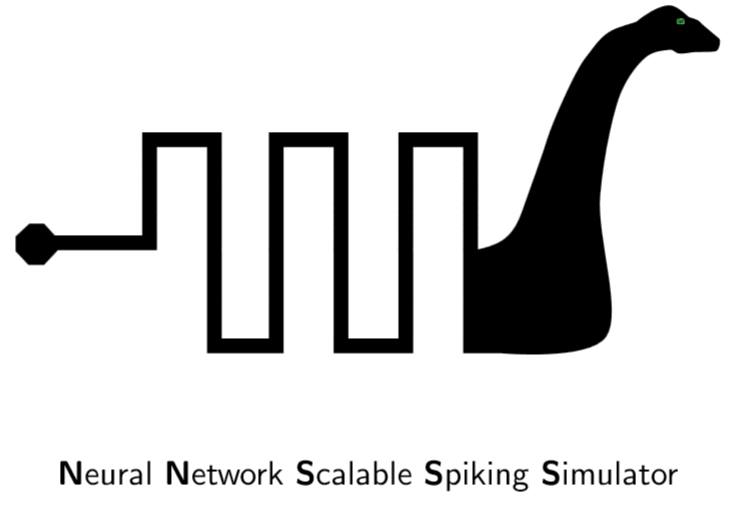
\includegraphics[scale=0.4]{image/n2s3.jpg}

\vfill
{\LARGE
\noindent
	Benjamin \textsc{Danglot}\newline
	Pierre \textsc{Falez}
}

\vfill
{
\noindent
{\LARGE Tuteur : Pierre Boulet} \hfill Sujet n°65 PJI 2015 
}

\newpage

%Remerciements

\section*{Remerciements}

Nous souhaitons remercier Pierre Boulet, Mahyar Shahsavari et Philippe Devienne, qui nous ont accompagné durant notre PJI.

\newpage

% Table of contents

\tableofcontents

\newpage

% Introduction

\section*{Introduction}

\subsection*{Sujet} 

\paragraph{}
Dans le cadre de notre PJI, nous avons choisi le sujet 65 intitulé \enquote{Environnement de simulation d'un accélérateur neuromorphique}. Ce dernier consiste à travailler sur la conception d'un simulateur en remplissant deux objectifs principaux : créer un langage dédié à la description d'architectures de réseaux de neurones et créer un langage de description d'un ensemble de simulations.

\paragraph{}
Cependant, le projet a eu d’autres besoins plus urgents, et nous avons donc développé d'autres fonctionnalités.

\subsection*{Motivations}
Dans notre volonté de faire un doctorat, nous pensons que ce sujet était particulièrement approprié pour nous apprendre des aspects de la recherche. De plus, l’utilisation de Scala, et donc de son apprentissage était également un apport majeur à notre culture informatique. Nous avons également pu découvrir une part de la bio-informatique, ainsi qu'une nouvelle technologie de pointe, qui sera omniprésente : le memristor.


% Project presentation
\newpage

\section{Présentation du projet}

\subsection{Technologies}

\paragraph{}
Nous avons dû être confrontés à des technologies nouvelles pour nous tout au long de ce projet. Nous avons donc eu une phase d'apprentissage avant de pouvoir réellement commencer le projet.

\subsubsection{Scala} 
\begin{figure}[h!]

\includegraphics[scale=0.15,right]{image/scala.png}
\end{figure}
\paragraph{}
Scala est un langage de programmation multi-paradigme créée par l’École polytechnique fédéral de Lausanne (EPFL). Il combine la programmation orientée objet et la programmation fonctionnelle. Le langage Scala permet également de passer à l’échelle, et le fait qu’il utilise la machine virtuelle Java (JVM) permet une portabilité sur différentes plateformes et ainsi l’utilisation de cluster pour fonctionner.

\subsubsection{Akka} 
\begin{figure}[h!]

\includegraphics[scale=0.1,right]{image/akka.png}
\end{figure}
\paragraph{}
Akka est une bibliothèque disponible en Java et Scala qui permet d’ajouter de la concurrence et de la distribution, via un système d'acteur et de message.
        
\subsubsection{JspikeStack} 

\paragraph{}
JspikeStack est une application écrite en Java basée sur le modèle d'une machine de Boltzmann restreinte, qui construit et simule un réseau neuronal. Celui-ci permet notamment d’utiliser des réseaux pré appris, par exemple Mnist, qui reconnaît les chiffres écrits manuellement via une caméra DVS (Dynamic Vision Sensor)

\subsubsection{Memristor} 
\begin{figure}[h!]
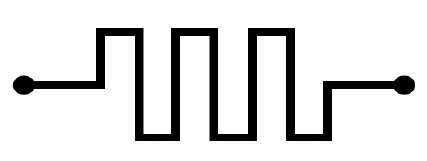
\includegraphics[scale=0.12,right]{image/memristor.jpg}
\end{figure}
\paragraph{}
Les memristors sont des composants électroniques dits passifs. Ce mot vient de la contraction de “memory” et “resistance”. Ce composant utilise sa résistance qui peut varier grâce à un courant électronique pour stocker de l’information. Le memristor a été “prédit” en 1971 par Leon Chua, mais le premier exemplaire physique n’a vu le jour qu’en 2008 par une équipe de chercheurs des laboratoires HP. Les memristors peuvent émuler le comportement d'une synapse biologique, d’où l’implémentation d’un simulateur pour étudier le comportement de ces nouveaux composants.

\newpage

\subsection{État actuel}

\paragraph{}
Notre PJI est la suite directe d’un PJI entamé l’année dernière, ainsi que d’un projet M2. Nous avons donc pu rencontrer les étudiants qui ont démarré le projet, et ainsi avoir une présentation de leurs travaux.

\paragraph{}
Il s’agit de l’implémentation d’un simulateur de neurones à base d'impulsions, les messages que s’échangent les neurones grâce aux synapses par lesquelles ils sont reliés. Il y a plusieurs simulateurs déjà existants, mais qui  ont chacun certains défauts, notamment le passage à l’échelle, et donc une limitation dans les performances de simulation\footnote{par exemple BRIAN, développait en python. L'utilisation du python limite le nombre de neurones pouvant être utilisés}. Le projet est baptisé N2S3 (Nessie) : \emph{\textbf{N}eural \textbf{N}etwork \textbf{S}calable
\textbf{S}pike \textbf{S}imulator}.

\paragraph{}
Lorsque nous avons repris le projet, ce dernier avait déjà certaines fonctionnalités partiellement ou complètement opérationnelles.

\paragraph{}
Le projet a été pensé de façon générique : il doit pouvoir s’adapter à différent modèle de réseau. Pour le moment seul, le modèle QBG (Querlioz - Bichler - Gamrat) est implémenté. C’est pourquoi le projet est réparti dans différents packages de la façon suivante :

\begin{itemize}
	\item un package \emph{core} contient les classes génériques pour représenter un réseau.
	\item un package \emph{feature.io} pour toutes les fonctionnalités d’entrées/sorties.
	\item un package \emph{feature.logging} pour la gestion des logs.
	\item un package \emph{models.qbg} pour implémenter un réseau de ce type.
\end{itemize}

\paragraph{}
L’implémentation du réseau a été pensée de la manière suivante : chaque neurone et chaque synapse sont représentés par un acteur. Un synchroniseur, qui est également  un agent, est en charge de récupérer tous les messages, et de les redistribuer à travers le réseau pour que la cohérence dans le temps soit bien respectée.
\newpage
\paragraph{}
Les neurones sont répartis dans différentes couches. Comme le simulateur pour le moment suit le modèle restreint de machine de Boltzmann, les seules communications entre les neurones se font entre des couches voisines. Il n'y a donc pas non plus d’interconnexion entre des neurones d'une même couche. Ceci permet de faciliter les mécanismes de synchronisation temporels.

\begin{figure}[h!]
\centering
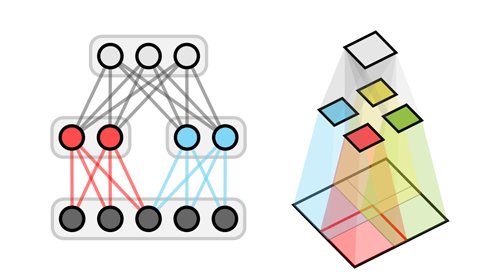
\includegraphics[scale=0.4]{image/boltzmann.png}
\caption{Exemple d'un réseau suivant le modèle de machine de Boltzmann}
\end{figure}

\paragraph{}
Avec le modèle actuel, chaque neurone possède un potentiel qui, lorsqu'il dépasse un seuil fixé, va envoyer des impulsions à l'ensemble des neurones qui sont reliés avec lui. Chaque synapse possède un poids synaptique qui varie au cours de la simulation. Ce poids augmente lorsque le neurone réenvoie une impulsion dans une certaine fenêtre de temps après qu'une autre impulsion est passée dans cette synapse. Si le neurone de renvoie rien, alors le poids diminue. Pour reproduire ce comportement, différents types d'impulsions qui sont implémentés par des messages, ont été créés : 
\begin{itemize}
\item \emph{PreSynapticSpike} qui est le message envoyé par un neurone vers une synapse
\item \emph{PostSynapticForwardSpike} qui est le message envoyé par une synapse vers un neurone. Cette dernière transmet son propre poids synaptique au neurone.
\item \emph{PostSynapticBackwardSpike} qui est le message renvoyé par le neurone vers ses synapses lorsque son potentiel a dépassé le seuil fixé. Celui-ci est nécessaire pour affecter le poids synaptique en fonction de la réaction du neurone.
\end{itemize}

\paragraph{}
Pour commencer la simulation, il suffisait de lancer des messages dans le réseau sur des neurones afin de les stimuler et de propager les impulsions aux couches supérieures.

\newpage
\subsection{Perspectives du travail réalisé}
\paragraph{}
Le simulateur fonctionne globalement, mais certains aspects été à revoir :
\begin{itemize}
\item La fourniture à la main d’entrées dans le simulateur n’est pas une solution convenable, de même que la création manuelle d’un réseau neuronal.
\item Les visualisations actuelles ne sont pas satisfaisantes, et les logs ne permettent pas de bien comprendre l’évolution du réseau.
\item Avec un unique synchroniseur pour le simulateur, le passage à l’échelle est impossible. Celui-ci devient un goulot d’étranglement et ralentit toute la progression de la simulation.
\item Il est nécessaire de repenser l'architecture globale du projet afin de bien séparer les différentes expérimentations des différents modèles de réseau.
\end{itemize}

\paragraph{}
Nous avons donc travaillé sur ces points, afin de permettre à N2S3 d’évoluer.

\newpage

\section{Ajout des entrées}

\paragraph{}
Notre première tâche dans ce projet fut de mettre en place un système d'entrées afin de pouvoir stimuler le réseau. Celle-ci fut une bonne introduction pour nous, car elle nous a permis de prendre en main et d’aborder pas à pas le projet.

\paragraph{}
Les fichiers JAER contiennent les données produites, par exemple, par une caméra DVS. Ce fichier se présente sous la forme d’une liste d’événements. Chaque événement étant représenté par un temps et une source. Ainsi, notre tuteur avait déjà implémenté une classe qui lit ces fichiers à partir d’une librairie ajoutée à N2S3. 

\paragraph{}
Pour gérer ces événements d’entrées, nous avons créé une classe abstraite (Annexe \ref{input_generator}) dont l’implémentation dépendra du format de fichier d’entrée. Étant donné que nous avions à notre disposition des fichiers JAER, et une classe de lecture, nous avons directement ajouté une classe pour ces formats de fichiers.

\paragraph{}
Cette classe se chargera de lire et d'envoyer les événements ordonnés temporellement. Dans les premières versions, la gestion des entrées était totalement “indépendante” du réseau. Tant qu’il y avait des entrées dans le fichier, elles étaient envoyées au synchroniseur. Mais cette méthode le surchargeait, et donc ralentissait l’évolution du réseau. À présent, le synchroniseur demande de nouvelles entrées lorsqu’il juge qu’il en a besoin (lorsque le nombre de messages dans sa file d'événements passe en dessous d'un certain seuil). Nous avons également dû faire attention d'envoyer en une seule fois tous les événements du fichier produits au même moment afin d'éviter tout conflit de causalité.

\newpage

\section{Création de réseau à partir de fichier XML}

\paragraph{}
Nous avons ensuite développé une classe qui permet de créer un réseau neuronal à partir d’un fichier XML.
Nous avons pris comme base, les fichiers XML utilisés par Peter O’Connor dans sa thèse (Annexe \ref{xml_exemple}). La classe permet d’initialiser le réseau, de connecter les neurones et les synapses ainsi que de leur affecter des potentiels/seuils à l’initialisation.

\paragraph{}
Ce fichier est construit de la manière suivante. L'ensemble du réseau est décrit à l'intérieur de la balise \emph{Network}. On retrouve notamment le nom du réseau, son type, le nombre de couches ainsi que des paramètres optionnels (température, fréquence de mise à jour, etc.). Puis pour chaque couche, il y a une balise \emph{Layer} contenant la description de cette dernière. Chaque couche est identifiée par un index, via la balise \emph{index}. Elle possède également une couche cible, \emph{targ}, qui est la couche de sortie avec laquelle ses neurones sont connectés. De plus, \emph{nUnits} donne le nombre de neurone contenu dans la couche courante et \emph{dimx} \emph{dimy} leurs répartitions sur un plan à deux dimensions. Enfin, chaque seuil des neurones de la couche est représenté par un flottant simple précision encodé sous forme de base 64 dans la balise \emph{thresh} et de la même manière chaque poids synaptique est encodé dans la balise \emph{W}. Comme on travaille avec des modèles de machine de Boltzmann, les neurones entre deux couches voisines sont reliés de façon complète : chaque neurone possède une connexion vers l'ensemble des neurones de la couche voisine.

\paragraph{}
Pour réaliser cette fonctionnalité, nous avons utilisé la bibliothèque XML directement intégrée à Scala. Nous récupérons dans un premier temps le nombre de couches et le nombre de neurones pour chaque couche ainsi que la topologie de ces dernières. À partir de ces informations, nous construisons et initialisons le réseau. Nous avons ensuite créé des messages afin de pouvoir modifier les paramètres des neurones et des synapses (leurs seuils et leurs poids synaptiques). Enfin, nous avons décodé puis transmis ces paramètres pour chaque neurone et chaque synapse. (Annexe \ref{xml_builder})

\newpage
\section{Amélioration du synchroniseur}

\subsection{Gestion de l'état du synchroniseur}

\paragraph{}
Avec l'ajout de gestion des entrées, nous avons été confrontés au problème de savoir qui contrôle le flux d’événement. Il est naturel que ce soit le synchroniseur qui contrôle l’approvisionnement sur les entrées est non l'inverse. Nous avons donc fait en sorte d'associer une entrée au synchroniseur afin que ce dernier puisse demander de nouveaux événements lorsqu'il en a besoin. Ceci permet à la fois de stopper ou reprendre l’exécution de la simulation assez facilement, mais surtout d'éviter de sous-charger ou de surcharger le synchroniseur en éventement.

\paragraph{}
Avec ce système, il est maintenant nécessaire de créer l'entrée indépendamment du réseau, puis de lier cette dernière au synchroniseur. Il suffit ensuite simplement d'envoyer des messages de contrôle au synchroniseur : \emph{Start} pour déclencher l’exécution de la simulation, \emph{Step} pour envoyer un unique événement d'entré et \emph{Stop} pour terminer cette dernière

\subsection{Utilisation de plusieurs synchroniseurs}

\paragraph{}
Pour améliorer la mise à l'échelle du simulateur, nous avons réfléchi à utiliser plusieurs synchroniseurs afin de répartir la transition des messages et ainsi gagner en parallélisme. Le principal problème qui survient lors de l'utilisation de synchroniseur indépendant les uns des autres est que des problèmes de causalité temporelle peuvent survenir. Néanmoins, l'utilisation du modèle de machine de Boltzmann réduit  permet séparer le réseau en différente couche. De plus, on considère pour le moment que le réseau ne comporte pas de boucle, et donc que les couches peuvent être indépendantes temporellement.

\paragraph{}
Une des premières taches fut de rendre la création du synchroniseur générique. Pour cela, nous avons créé une classe abstraite qui permet de cacher l'initialisation et la récupération du synchroniseur concerné. Nous avons étendu cette classe avec deux implémentations : La première créer un unique synchroniseur et le retourne pour l'ensemble des acteurs du réseau et la seconde qui créer un synchroniseur par couche et renvoi le bon en fonction de la couche de l'acteur concerné.

\paragraph{}
Cependant, il reste quelques problèmes de causalité à résoudre, notamment dus au fait que les neurones renvoient un message aux synapses pour affecter leurs poids synaptiques.

\newpage

\section{Génération de graphes}

\paragraph{}
Nous avons mis en place une génération de graphe à partir des fichiers de log créés par chacun des acteurs. En effet, pour pouvoir apprécier les simulations et leurs résultats, une visualisation graphique est nécessaire.
Celle-ci s'effectue généralement en deux passes : 

\begin{itemize}
	\item{1}: La lecture du fichier de log et la création de variables qui permettent de configurer correctement les fichiers qui seront générés.
	\item{2}: La génération en elle-même, qui crée deux fichiers : un fichier de données contenant toutes les informations que le graphe a besoin pour répondre au besoin de l'utilisateur, et un fichier plot, qui utilise ce fichier de données et les variables définies durant la lecture.
\end{itemize}
(Annexe \ref{gen_graph})

\subsection{Graphes d’activité des neurones}
\paragraph{}
À partir des logs que les neurones créent, nous pouvons générer un graphe d’activité neuronale. 

\begin{figure}[!h]
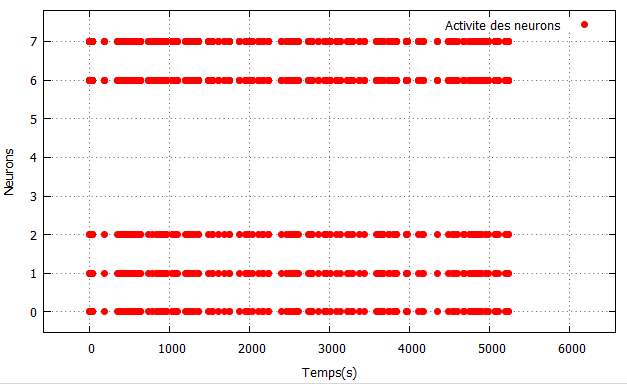
\includegraphics[scale=0.75,right]{image/neuronActivity.png}
\caption{Activité des neurones en fonction du temps.}
\end{figure}

\paragraph{}
Certaines options sont disponibles pour générer ce type de graphes :
\begin{itemize}
\item{Donner la liste des index des neurones que l’on souhaite observer.}
\item{Donner la liste des index des couches que l’on souhaite observer.}
\item{Donner un temps maximum.}
\end{itemize}

\subsection{Graphes des activités des synapses}

De même que pour les neurones, on peut observer l'évolution des poids synaptiques du réseau.

\begin{figure}[!h]
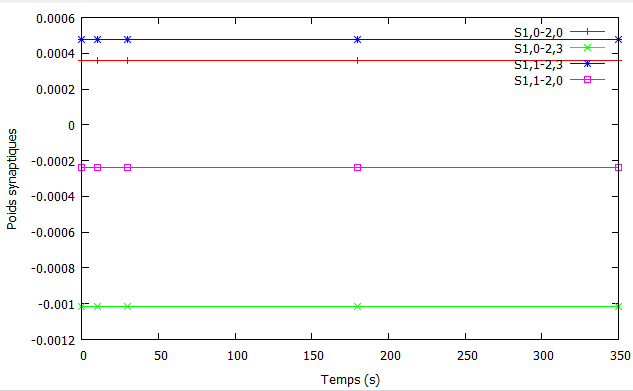
\includegraphics[scale=0.75,right]{image/synapsesActivity.png}
\caption{Poids synaptiques avec la couche 1 en entrée en fonction du temps.}
\end{figure}

\subsubsection*{Remarques}
\paragraph{}
Ces générations se font pour l’instant sur de petits exemples de fichiers de logs, mais il faut l’améliorer  pour pouvoir avoir des visualisations sur de véritables simulations, avec des réseaux de l’ordre de millions de neurones.
De plus, les exemples de logs utilisés ne sont pas significatifs.

\newpage

\section*{Conclusion}

\subsection*{Bénéfice de l'expérience}
\subsubsection*{Scolaire}
Bien que nous ayons déjà travaillé ensemble, le PJI nous a permis de renforcer notre travail d'équipe, ainsi que d'apprendre  le Scala, qui est un langage extrêmement puissant. Nous avons également pu pratiquer la programmation fonctionnelle, chose que l'ont à peu l'occasion de faire durant notre scolarité, mais également le concept d'agent / messages.

\subsubsection*{Professionnel}
Nous avons pu durant ce projet, faire nos premiers pas dans la recherche, découvrir le fonctionnement interne d'une équipe, ce qui nous a beaucoup plu et conforté dans l'idée de poursuivre nos études après le master. Travailler sur un logiciel destiné à faire avancer la recherche est une source de motivation conséquente.

\subsubsection*{Humain}
Le projet nous a permis de rencontrer des personnes intéressantes. Nous avons pu dégager un contrat avec l'équipe pour continuer de travailler cet été sur N2S3.

\subsection*{L'avenir du projet}
N2S3 possède un grand potentiel, qui demande encore des efforts de développement, notamment sur la visualisation des simulations ainsi que sur le passage à l'échelle.

\newpage

\appendix
\section{Génération de graphes}
Exemples de code pour la génération de graphes de l'activité neuronale.
\label{gen_graph}
Boucles pour construire le fichier de données.
\lstinputlisting[style=Scala_style]{src/loopdata.scala}
Génération du fichier plot
\lstinputlisting[style=Scala_style]{src/pltgen.scala}
\subsection{Exemple de fichier de graphe (gnuplot)}
Voici un exemple de fichier plot généré grâce à l'application, il concerne l'activité neuronale du réseau : 
\lstinputlisting[breaklines=true]{src/neurons.plt}

\section{Classe abstraite de gestion des entrées}
\label{input_generator}
\lstinputlisting[style=Scala_style]{src/InputGenerator.scala}

\section{Exemple de fichier xml}
\label{xml_exemple}

Voici l'exemple du fichier XML utilisé par Peter O'Connor dans sa thèse, sur lequel nous avons bâti notre constructeur de réseau à partir de fichier XML :
 
\lstinputlisting[style=XML_style]{src/example.xml}

\section{Code du générateur de réseau via fichier XML}
\label{xml_builder}
\lstinputlisting[style=Scala_style]{src/XMLBuilder.scala}

\end{document}